\documentclass[aspectratio=169]{beamer}
	\usepackage[utf8]{inputenc}		% required for umlauts
	\usepackage[english]{babel}		% language
	%\usepackage[sfdefault]{roboto}	% enable sans serif font roboto
	%\usepackage{libertine}			% enable this on Windows to allow for microtype
	\usepackage[T1]{fontenc}		% required for output of umlauts in PDF

	\usepackage{mathtools}		% required for formulas

	\usepackage{caption}		% Customize caption aesthetics
	\usepackage{tcolorbox}		% fancy colored boxes
	\usepackage{xcolor}			% Highlighting
	\usepackage{soul}

	\usepackage{graphicx}		% required to insert images
	\usepackage{subcaption}		% enable sub-figure
	\usepackage[space]{grffile} % insert images baring a filename which contains spaces
	\usepackage{float}			% allow to forcefully set the location of an object

	\usepackage[tracking=true]{microtype} % required to change character spacing

	\usepackage[style=numeric,backend=biber]{biblatex}
	\usepackage{hyperref}		% insert clickable references

	\usepackage{datetime}		% flexible date specification
	\newcommand{\leadingzero}[1]{\ifnum#1<10 0\the#1\else\the#1\fi}
	\newcommand{\todayddmmyyyy}{\leadingzero{\day}.\leadingzero{\month}.\the\year}
	\newcommand{\mathcolorbox}[2]{\colorbox{#1}{$\displaystyle #2$}}

	\usepackage{geometry}
	\usepackage{scrextend}		% allow arbitrary indentation

	\usepackage{color}

	\setbeamercolor{title}{fg=orange}
	\setbeamertemplate{title}{
		\color{orange}
		\textbf{\inserttitle}
	}
	\setbeamercolor{tableofcontents}{fg=orange}
	\setbeamercolor{section in toc}{fg=black}
	\setbeamercolor{subsection in toc}{fg=black}
	\setbeamertemplate{frametitle}{
		%\vspace{0.5em}
		\color{orange}
		\begin{center}
			\textbf{\insertframetitle} \\
			{\small \insertframesubtitle}
		\end{center}
	}
	\setbeamertemplate{footline}[text line]{
  		\parbox{\linewidth}{
			  \color{gray}
			  \vspace*{-1em}
			  PSRC 2018
			  \hfill
			  Gordian (\href{mailto:gordian.edenhofer@gmail.com}{gordian.edenhofer@gmail.com})
			  \hfill
			  \insertpagenumber
		}
	}
	\setbeamertemplate{navigation symbols}{}
	\setbeamertemplate{itemize item}{\color{black}$\bullet$}
	\setbeamertemplate{itemize subitem}{\color{black}$\circ$}
	\setbeamercolor{block title}{fg=black}
	\captionsetup{font=scriptsize,labelfont={bf,scriptsize}}

	\title{Seventh Weekly Update on `Optimization~of~Particle~Identification'}
	\subtitle{Neyman Pearson by detector, pt and cosTheta; Abundance comparisons; Neural Network for different optimizers and various parameters}
	\author[Edenhofer]{\href{mailto:gordian.edenhofer@gmail.com}{Gordian Edenhofer}}
	\institute[LMU]{
		Working Group of Prof.~Dr.~Kuhr \\
		Faculty of Physics \\
		Excellence Cluster Universe
	}
	\date[BA Thesis 2018]{\today}
	\subject{Particle Physics}


\begin{document}
\section{Git log}
\begin{frame}
	\frametitle{\insertsection}

	\begin{itemize}
		\item Neyman Pearson
		\begin{itemize}
			\item{By pt (\textit{Appendix})}
			\item{By cosTheta (\textit{Appendix})}
		\end{itemize}
		\item Abundance comparisons
		\item Neural Network
		\begin{itemize}
			\item{By optimizer}
			\item{By batch size}
		  \end{itemize}
	\end{itemize}
\end{frame}

\section{Neyman Pearson}
\subsection{Anomalies}
\begin{frame}
	\frametitle{\insertsection}
	\framesubtitle{\insertsubsection}

	\begin{figure}
		\centering
		\begin{subfigure}{0.49\textwidth}
			\centering
			\includegraphics[width=\textwidth,height=0.7\textheight,keepaspectratio]{{{../res/charged 01/General Purpose Statistics: Relative p Abundance in Likelihood Ratio Bins for ALL detector}}}
			\caption{`ALL' detector}
		\end{subfigure}
		\begin{subfigure}{0.49\textwidth}
			\centering
			\includegraphics[width=\textwidth,height=0.7\textheight,keepaspectratio]{{{../res/charged 01/General Purpose Statistics: Relative p Abundance in Likelihood Ratio Bins for CDC detector}}}
			\caption{`CDC' detector}
		\end{subfigure}

		\caption{Relative $p$ abundance in likelihood ratio bins for various detectors.}
	\end{figure}
\end{frame}

\section{Abundance comparisons}
\begin{frame}
	\frametitle{\insertsection}
	\framesubtitle{\insertsubsection}

	\begin{figure}
		\centering
		\begin{subfigure}{0.49\textwidth}
			\centering
			\includegraphics[width=\textwidth,height=0.7\textheight,keepaspectratio]{{{../res/charged 01/Diff Abundances: Particle Abundances in the K+-Data via PID, via flat Bayes}}}
			\caption{PID, flat Bayes}
		\end{subfigure}
		\begin{subfigure}{0.49\textwidth}
			\centering
			\includegraphics[width=\textwidth,height=0.7\textheight,keepaspectratio]{{{../res/charged 01/Diff Abundances: Particle Abundances in the K+-Data via flat Bayes, by pt & cos(Theta)}}}
			\caption{flat Bayes, by $p_t$ \& $\cos(\Theta)$}
		\end{subfigure}

		\caption{Particle Abundances for different selection method with an exclusive classification.}
	\end{figure}
\end{frame}

\section{Neural Network by optimizer}
\subsection{Fair sampling}
\begin{frame}
	\frametitle{\insertsection}
	\framesubtitle{\insertsubsection}

	\begin{figure}
		\centering
		\begin{subfigure}{.32\textwidth}
			\centering
			\includegraphics[width=\textwidth,height=0.26\textheight,keepaspectratio]{{{../res/sample/Neural Network Model: Accuracy pca fair nLayers7 Optimizerrmsprop LearningRateNone nEpochs20 BatchSize192}}}
			\caption{RMSprop}
		\end{subfigure}
		\begin{subfigure}{.32\textwidth}
			\centering
			\includegraphics[width=\textwidth,height=0.26\textheight,keepaspectratio]{{{../res/sample/Neural Network Model: Accuracy pca fair nLayers7 Optimizeradagrad LearningRateNone nEpochs20 BatchSize192}}}
			\caption{Adagrad}
		\end{subfigure}
		\begin{subfigure}{.32\textwidth}
			\centering
			\includegraphics[width=\textwidth,height=0.26\textheight,keepaspectratio]{{{../res/sample/Neural Network Model: Accuracy pca fair nLayers7 Optimizeradadelta LearningRateNone nEpochs20 BatchSize192}}}
			\caption{Adadelta}
		\end{subfigure}

		\begin{subfigure}{.32\textwidth}
			\centering
			\includegraphics[width=\textwidth,height=0.26\textheight,keepaspectratio]{{{../res/sample/Neural Network Model: Accuracy pca fair nLayers7 Optimizeradam LearningRateNone nEpochs20 BatchSize192}}}
			\caption{Adam}
		\end{subfigure}
		\begin{subfigure}{.32\textwidth}
			\centering
			\includegraphics[width=\textwidth,height=0.26\textheight,keepaspectratio]{{{../res/sample/Neural Network Model: Accuracy pca fair nLayers7 Optimizeradamax LearningRateNone nEpochs20 BatchSize192}}}
			\caption{Adamax}
		\end{subfigure}
		\begin{subfigure}{.32\textwidth}
			\centering
			\includegraphics[width=\textwidth,height=0.26\textheight,keepaspectratio]{{{../res/sample/Neural Network Model: Accuracy pca fair nLayers7 Optimizernadam LearningRateNone nEpochs20 BatchSize192}}}
			\caption{Nadam}
		\end{subfigure}

		\caption{Accuracy by optimizer for a PCA feature selection and using fair sampling.}
	\end{figure}
\end{frame}

\subsection{Biased sampling}
\begin{frame}
	\frametitle{\insertsection}
	\framesubtitle{\insertsubsection}

	\begin{figure}
		\centering
		\begin{subfigure}{.32\textwidth}
			\centering
			\includegraphics[width=\textwidth,height=0.26\textheight,keepaspectratio]{{{../res/sample/Neural Network Model: Accuracy pca biased nLayers7 Optimizerrmsprop LearningRateNone nEpochs20 BatchSize192}}}
			\caption{RMSprop}
		\end{subfigure}
		\begin{subfigure}{.32\textwidth}
			\centering
			\includegraphics[width=\textwidth,height=0.26\textheight,keepaspectratio]{{{../res/sample/Neural Network Model: Accuracy pca biased nLayers7 Optimizeradagrad LearningRateNone nEpochs20 BatchSize192}}}
			\caption{Adagrad}
		\end{subfigure}
		\begin{subfigure}{.32\textwidth}
			\centering
			\includegraphics[width=\textwidth,height=0.26\textheight,keepaspectratio]{{{../res/sample/Neural Network Model: Accuracy pca biased nLayers7 Optimizeradadelta LearningRateNone nEpochs20 BatchSize192}}}
			\caption{Adadelta}
		\end{subfigure}

		\begin{subfigure}{.32\textwidth}
			\centering
			\includegraphics[width=\textwidth,height=0.26\textheight,keepaspectratio]{{{../res/sample/Neural Network Model: Accuracy pca biased nLayers7 Optimizeradam LearningRateNone nEpochs20 BatchSize192}}}
			\caption{Adam}
		\end{subfigure}
		\begin{subfigure}{.32\textwidth}
			\centering
			\includegraphics[width=\textwidth,height=0.26\textheight,keepaspectratio]{{{../res/sample/Neural Network Model: Accuracy pca biased nLayers7 Optimizeradamax LearningRateNone nEpochs20 BatchSize192}}}
			\caption{Adamax}
		\end{subfigure}
		\begin{subfigure}{.32\textwidth}
			\centering
			\includegraphics[width=\textwidth,height=0.26\textheight,keepaspectratio]{{{../res/sample/Neural Network Model: Accuracy pca biased nLayers7 Optimizernadam LearningRateNone nEpochs20 BatchSize192}}}
			\caption{Nadam}
		\end{subfigure}

		\caption{Accuracy by optimizer for a PCA feature selection and using biased sampling.}
	\end{figure}
\end{frame}

\section{Appendix}
\subsection{Anomalies in bins}
\begin{frame}
	\frametitle{\insertsection}
	\framesubtitle{\insertsubsection}

	\begin{figure}
		\centering
		\includegraphics[width=\textwidth,height=0.6\textheight,keepaspectratio]{{{../res/charged 01/pidProbability Approach: Relative p Abundance in Likelihood Ratio Bins for ALL detector for equal size pt bins}}}
		\caption{Relative $p$ Abundance in Likelihood Ratio Bins for the `ALL' detector using \textit{equal~height} $p_t$ bins.}
	\end{figure}
\end{frame}

\begin{frame}
	\frametitle{\insertsection}
	\framesubtitle{\insertsubsection}

	\begin{figure}
		\centering
		\includegraphics[width=\textwidth,height=0.6\textheight,keepaspectratio]{{{../res/charged 01/pidProbability Approach: Relative p Abundance in Likelihood Ratio Bins for ALL detector for equal size cos(Theta) bins}}}
		\caption{Relative $p$ Abundance in Likelihood Ratio Bins for the `ALL' detector using \textit{equal~height} $cos(\Theta)$ bins.}
	\end{figure}
\end{frame}

\begin{frame}
	\frametitle{\insertsection}
	\framesubtitle{\insertsubsection}

	\begin{figure}
		\centering
		\includegraphics[width=\textwidth,height=0.6\textheight,keepaspectratio]{{{../res/charged 01/pidProbability Approach: Relative p Abundance in Likelihood Ratio Bins for CDC detector for equal size pt bins}}}
		\caption{Relative $p$ Abundance in Likelihood Ratio Bins for the `CDC' detector using \textit{equal~height} $p_t$ bins.}
	\end{figure}
\end{frame}

\subsection{pidProbability scatter plot}
\begin{frame}
	\frametitle{\insertsection}
	\framesubtitle{\insertsubsection}

	\begin{figure}
		\centering
		\includegraphics[width=\textwidth,height=0.6\textheight,keepaspectratio]{{{../res/charged 01/General Purpose Statistics: p pidPropability multi-axes Histogram of pt, cosTheta above 0.05 Threshold}}}
		\caption{Multi-axes Histogram for the $p$-pidProbability above a 0.05 threshold as scatter plot depending on $p_t$ and $cos(\Theta)$.}
	\end{figure}
\end{frame}

\subsection{White paper of detector design}
\begin{frame}
	\frametitle{\insertsection}
	\framesubtitle{\insertsubsection}

	\begin{figure}
		\centering
		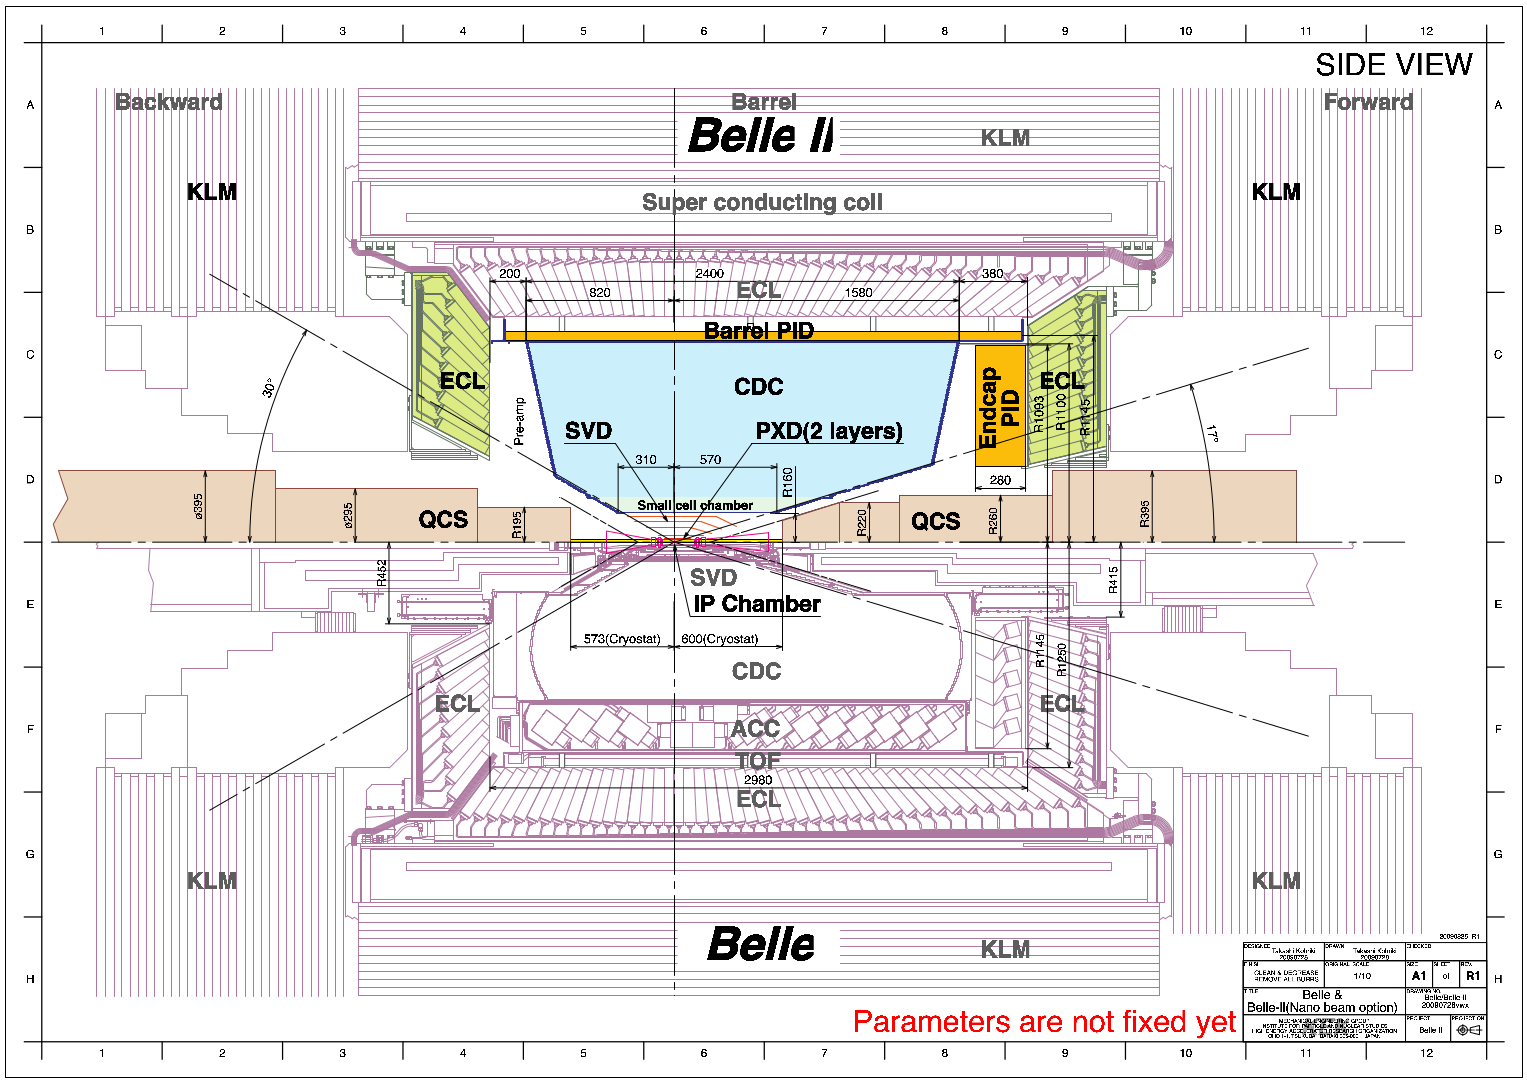
\includegraphics[width=\textwidth,height=0.65\textheight,keepaspectratio]{{{../res/Belle 2 detector design white paper}}}
		\caption{Belle 2 preliminary detector design at construction stage.}
	\end{figure}
\end{frame}

\end{document}
